 
% Appendix B

\chapter{Arquitectura del Sistema de Demostraci\'{o}n} % Main appendix title

\label{chapter:AppendixB} % For referencing this appendix elsewhere, use \ref{AppendixA}

Si bien el trabajo presentado no promete un sistema que implemente el mecanisno propuesto, es necesario tener un prototipo para demostrar el correcto funcionamiento del detector de anomal\'{i}as, por lo que este anexo se centra en presentar la arquitectura tanto f\'{i}sica como l\'{o}gica del prototipo.

\section{Arquitectura F\'{i}sica}

\begin{figure}[h!]
  \begin{center}	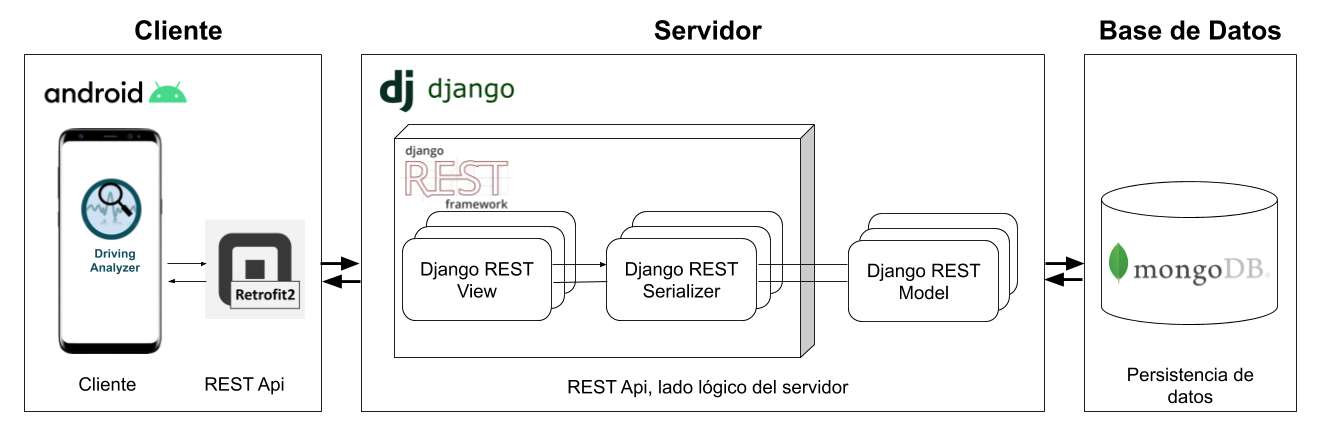
\includegraphics[width=0.95\textwidth, fbox]{imagenes/Apendices/Arquitectura}
  \caption{Arquitectura f\'{i}sica del Sistema de Demostraci\'{o}n (Elaboraci\'{o}n propia).}
  \label{fig:arq_fis}  
  \end{center}
\end{figure}

La arquitectura f\'{i}sica del prototipo cuenta con tres partes principales: el cliente, el servidor y la base de datos, como se puede observar en la Figura \ref{fig:arq_fis}. En primer lugar el cliente esta compuesto por una aplicaci\'{o}n m\'{o}vil para Android encargada de capturar los datos de los sensores inerciales, para posteriormente enviarlas al servidor usando Retrofit 2, posteriormente los datos ingresan al servidor realizado en Django, una vez el servidor recibe estos datos, se encarga de preprocesarlos para posteriormente predecir s\'{i} los datos enviados son anomal\'{i}as o no lo son, y por \'{u}ltimo los datos recibidos son almacenados en la Base de Datos de MongoDB con su respectiva predicci\'{o}n con el objetivo de hacer un monitoreo de la conducci\'{o}n del usuario.

\section{Arquitectura L\'{o}gica} 

\begin{figure}[h!]
  \begin{center}	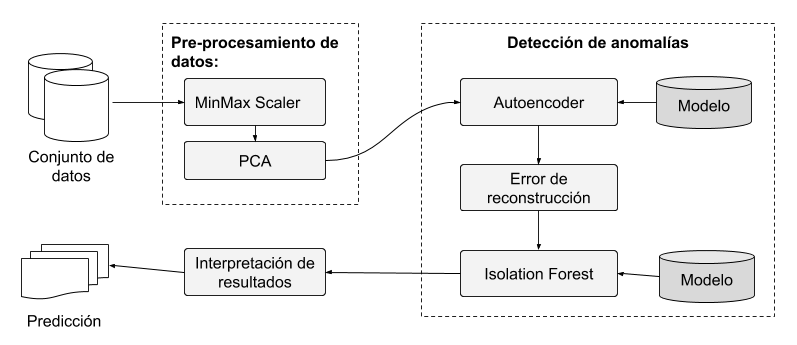
\includegraphics[width=0.95\textwidth, fbox]{imagenes/Apendices/arquitectura_logica}
  \caption{Arquitectura L\'{o}gica del Sistema de Demostraci\'{o}n (Elaboraci\'{o}n propia).}
  \label{fig:arq_log}  
  \end{center}
\end{figure}


En cuanto a la arquitectura l\'{o}gica se observa las dos principales partes del mecanismo de detecci\'{o}n propuesto: el pre-procesamiento y la detecci\'{o}n de anomal\'{i}as, como se puede observar en la Figura \ref{fig:arq_log}.